Στο σχήμα \ref{fig:wearAlongTrack} απεικονίζεται ο ρυθμός φθοράς κάθε ελαστικού (FL, FR, RL, RR) κατά μήκος της πίστας \textit{Circuit de Barcelona - Catalunya}, όπως προκύπτει από προσομοίωση ενός γύρου με τις παραμέτρους των \textit{Tremlett \& Limebeer} \cite{Tremlett2016} και χρήση του διαγράμματος \textit{GGV} σε ομοιόμορφη θερμοκρασία ελαστικών $80\,^\circ\mathrm{C}$. Έτσι διακρίνονται οι περιοχές της πίστας όπου συγκεντρώνεται η μεγαλύτερη φθορά για κάθε τροχό, καθώς και η διαφοροποίηση μεταξύ εμπρός/πίσω άξονα και εσωτερικού/εξωτερικού τροχού κατά τη διάρκεια των στροφών.\\[10pt]

\begin{figure}[htbp!]
    \centering
    \begin{subfigure}[t]{0.48\textwidth}
        \centering
        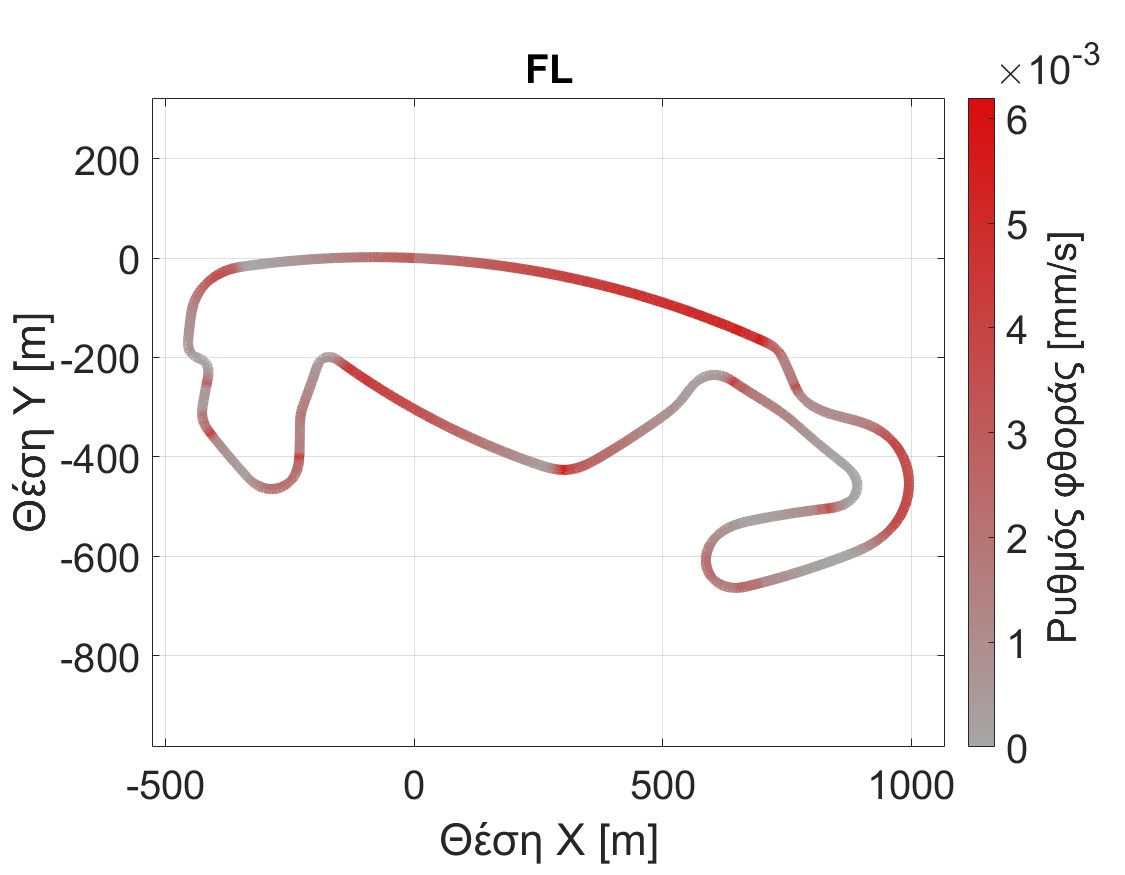
\includegraphics[width=\textwidth]{figures/wearAlongTrack_FL.jpg}
    \end{subfigure}
    \hfill
    \begin{subfigure}[t]{0.48\textwidth}
        \centering
        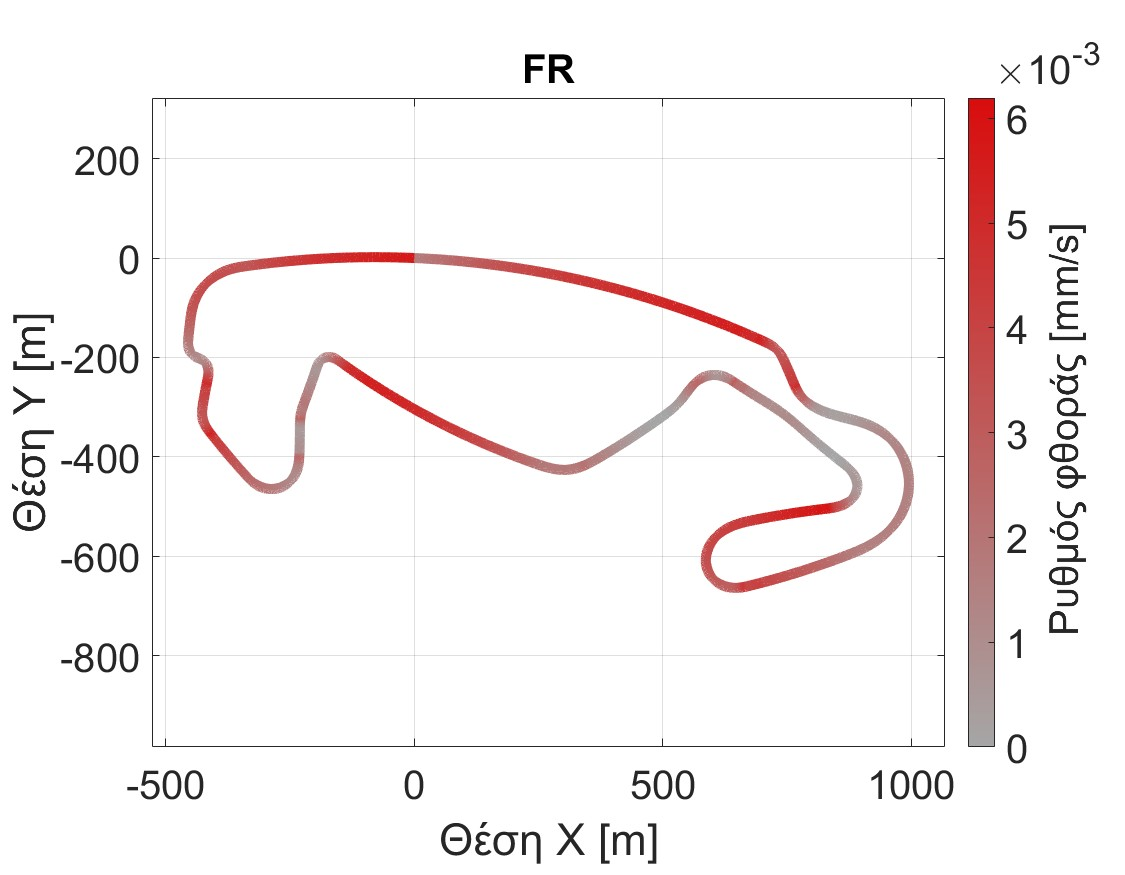
\includegraphics[width=\textwidth]{figures/wearAlongTrack_FR.jpg}
    \end{subfigure}

    \vspace{0.5em}

    \begin{subfigure}[t]{0.48\textwidth}
        \centering
        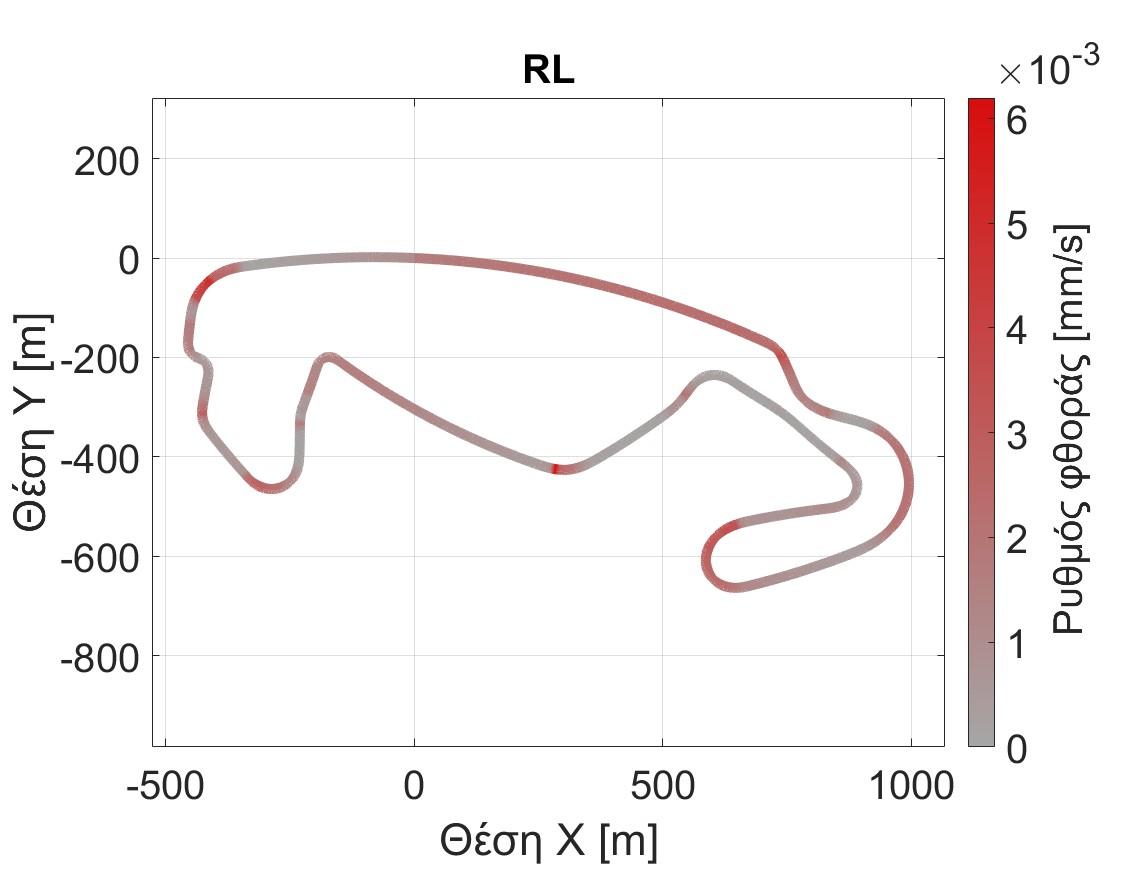
\includegraphics[width=\textwidth]{figures/wearAlongTrack_RL.jpg}
    \end{subfigure}
    \hfill
    \begin{subfigure}[t]{0.48\textwidth}
        \centering
        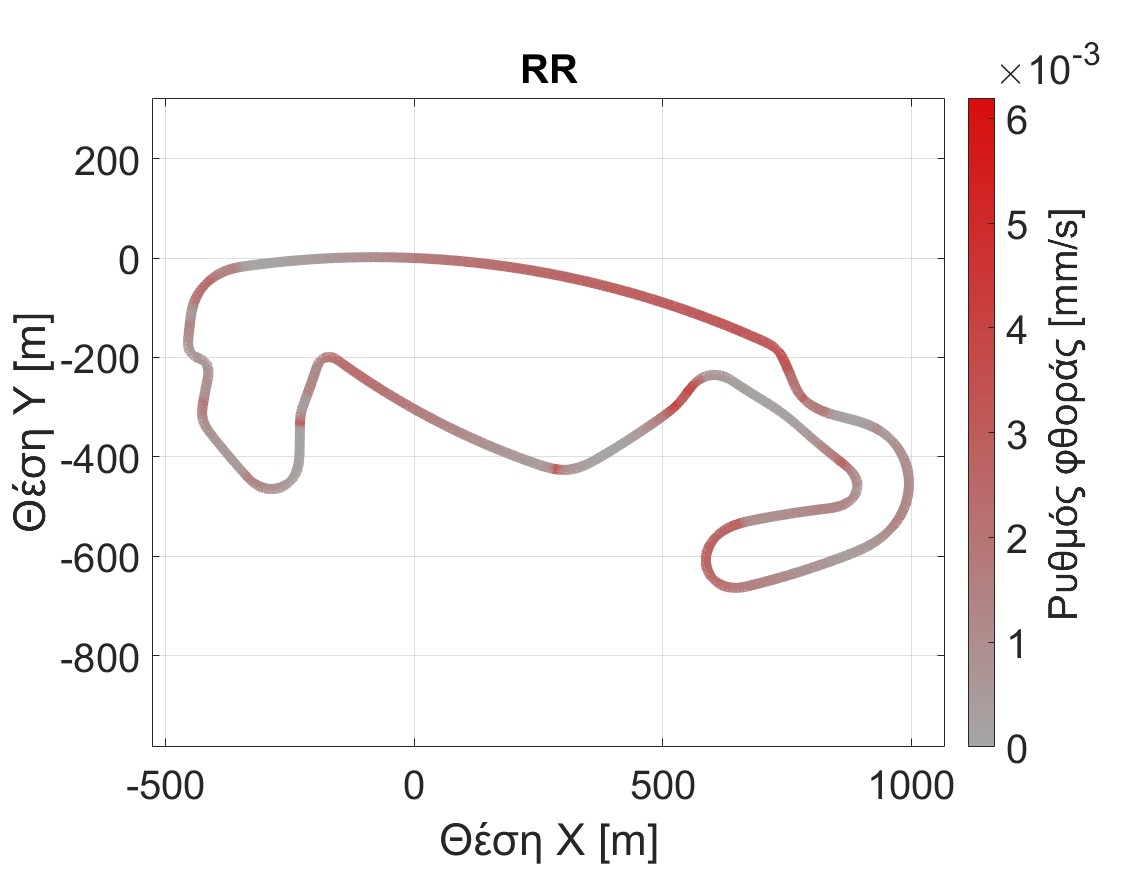
\includegraphics[width=\textwidth]{figures/wearAlongTrack_RR.jpg}
    \end{subfigure}
    \caption{Ρυθμός φθοράς κάθε ελαστικού κατά μήκος της πίστας \textit{Circuit de Barcelona - Catalunya}.}
    \label{fig:wearAlongTrack}
\end{figure}

\FloatBarrier
